\documentclass[010-intro.tex]{subfiles}

\begin{document}

\subsection{Computing Education (Higher Education)}

    The term ``computing'' is generally used to encompass all the various sub-fields that  have varying understandings and context
    \cite{cc2005, cc2020}.
    The original Computing Curricula 2005 Overview Report (for undergraduate education)
    addressed five (5) computing disciplines, which include: \cite{cc2005}:
    (1) computer engineering,
    (2) computer science,
    (3) information systems,
    (4) information technology, and
    (5) software engineering.
    Along with five (5) computational skills \cite{cc2005, cc2020}:
    (1) organizational system issues,
    (2) application technologies,
    (3) software development,
    (4) systems infrastructure, and
    (5) computer hardware and architecture.
    The interaction between computing disciplines and computational skills is reproduced in
    Figure \ref{fig:comp-disciplines-comp-skills},
    and was highly regarded in computing educational circles
    \cite{cc2005, cc2020}.
    The figure suggests that different computing disciplines require varying amount of computing skills,
    and as computing disciplines grow, new domains were added:
    cybersecurity in 2017, and
    data science in 2021
    \cite{ccdsc2021}.

    \begin{figure}[htb]
        \centering
        \includegraphics[width=0.9\textwidth]{figs/050-intro/cc/cc2005\_cc2020-visual-f3.2.PNG}
        \caption[Computational skills across computing disciplines]{
            The breakdown of how each of the 5 computational skills are utilized across each of the 5 computing disciplines.
            The 5 computational skills are
            organizational system issues, application technologies, software deveopment, systems infrastructure, and computer hardware and architecture.
            The 5 computational disciplines are
            computer engineering, computer science, information systems, infomational technology, and software engineering.
        }
        \label{fig:comp-disciplines-comp-skills}
    \end{figure}

    In addition to computing discipline changes,
    the learning frameworks on how to teach these disciplines have also changed
    from knowledge-based in 2005 to competency-based in 2020
    \cite{cc2020}.
    These learning framework changes stemmed from the discrepancy between
    skills taught in school that focus on individual tasks and skills needed for more complex real-world tasks
    \cite{cc2020}.
    The new computing curriculum guidelines released in 2020 are now as follows:

    \begin{enumerate}
        \item Focusing on competency
        \item Transitioning from knowledge-based learning to competency-based learning
        \item Expanding curricular disciplines to include cybersecurity as well as data science
        \item Expanding curricular and competency diagrams and visualizations
        \item Establishing an interactive website that will bring CC2020 results to public use
        \item Charting a framework for future computing curricular activities
    \end{enumerate}

    This dissertation explores computing skills required for data science,
    and how to build long-term competency for domain experts.
    The work also seeks to identify core data science competencies,
    and how to meet the existing skills gap for individuals who are not enrolled
    in a course program to learn these competencies.
    It aims to accomplish these tasks by
    testing and creating a framework for domain-specific set of materials in data science.

\subsection{Computing Education (K-12)}

    The Computer Science Teachers Association (CSTA)
    is a professional association aimed to support computer science teachers in K-12.
    Similar to the Computing Curriculum reports,
    the CSTA also has guidelines and standards for K-12 curriculums and teachers in computer science
    (Figure \ref{fig:csta-teaching-standards}) \cite{csta2017}.

    \begin{figure}[htb]
        \centering
        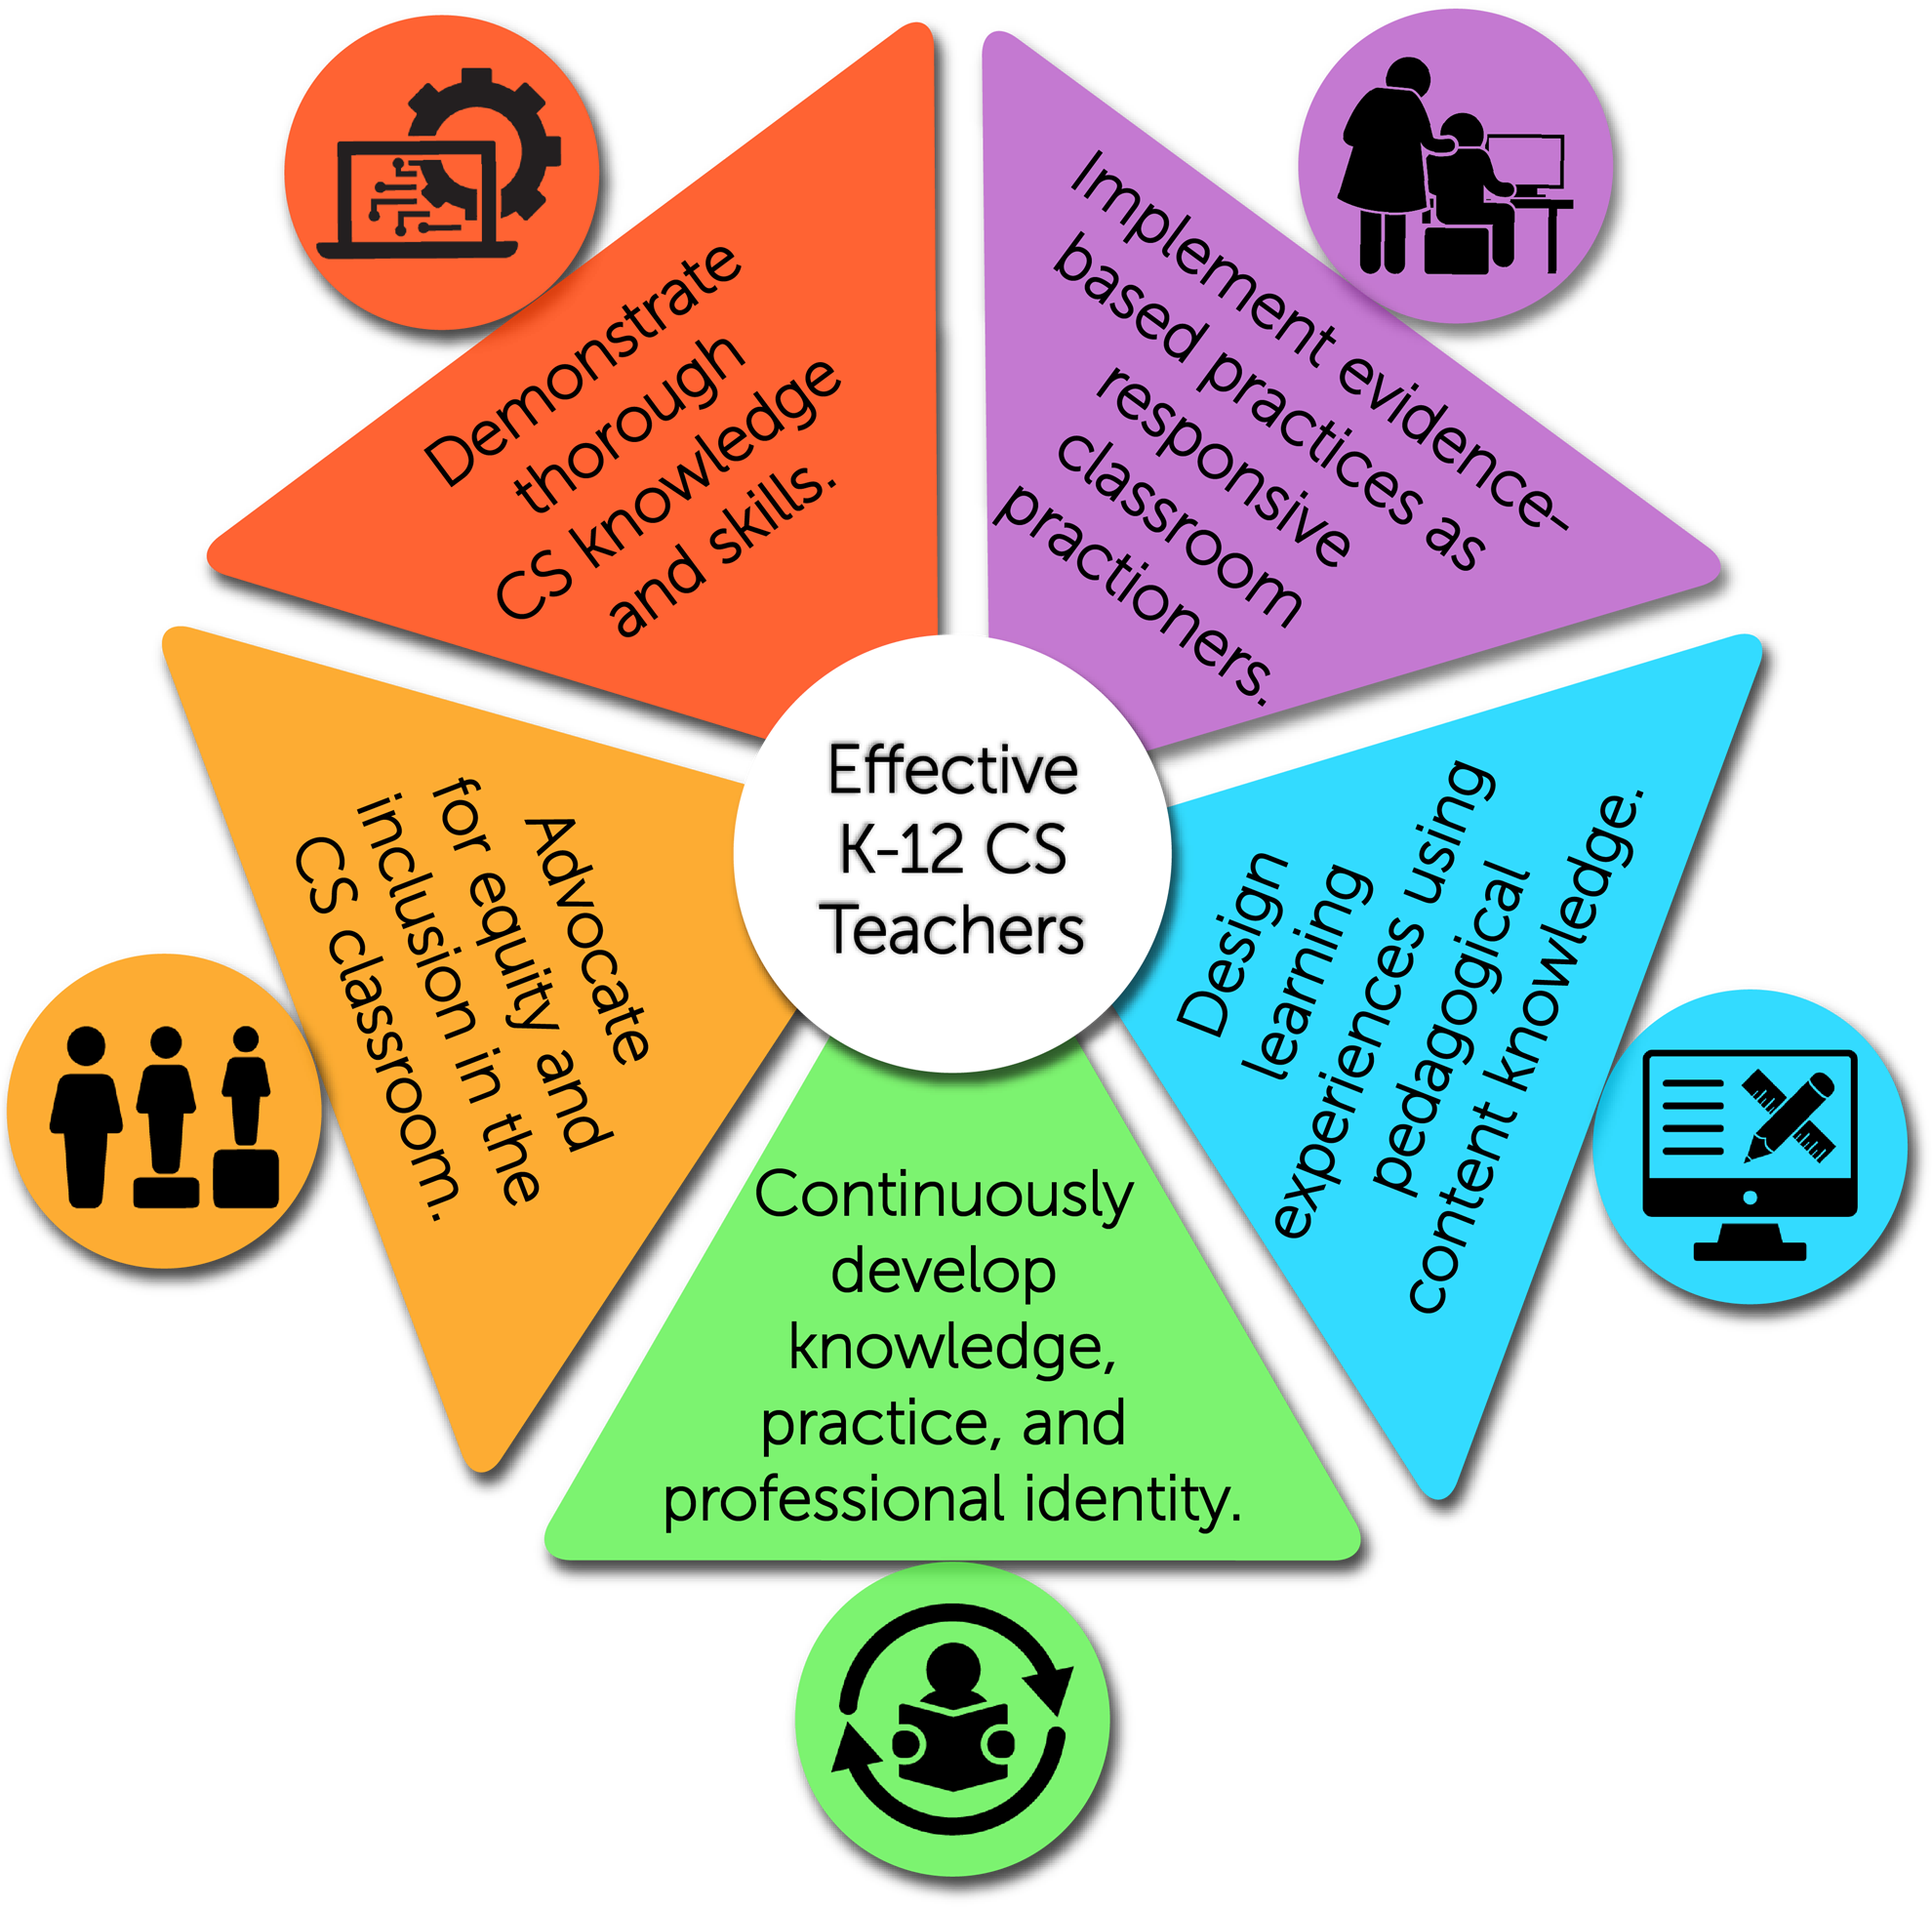
\includegraphics[width=0.6\textwidth]{figs/050-intro/CSTA-Standards-for-CS-Teachers---Main-Graphic.png}
        \caption[CSTA Standards for CS Teachers]{
            The 5 goals for effective K-12 computer science teachers.
            This figure is reproduced from the CSTA standards for CS teachers.
            Since CS teachers come from many different backgrounds,
            this figure lists the **** orient teachers to continuouly refine their pedagocial content knowledge (PCK).
            These goals help the teacher support the students in meeting learning outcomes.
            Many of these goals apply to teaching computational skills as well.
        }
        \label{fig:csta-teaching-standards}
    \end{figure}

    The CSTA standards are incorporating the need to understand computing literacy in K-12 edcation.
    The learning objectives for the standards fall into 5 main categories and have a progression (1A, 1B, 2, 3A and 3B)
    for students as they get older:
    (1) Computing Systems,
    (2) Networks and the Internet,
    (3) Data and Analysis,
    (4) Algorithms and Programming, and
    (5) Impacts of Computing.

    The CSTA learning standards align with the Computation Curriculum guidelines
    and its new focus around complex real-world jobs in undergraduate education with
    the CSTA guidelines in K-12 education in Data and Analysis,
    specifically,
    the CSTA 2-DA-08 standard for data analysis,
    ``collect data using computational tools and transform the data to make it more useful and reliable''
    \cite{csta, csta2017, cc2020}.

    This dissertation builds on the multiple computing reports by acknowledging data science as a separate computing discipline,
    and requires a different and adjacent set of computational skills
    from other computing disciplines,
    and aims to apply pedagogical best practices to effectively teach data science to specific domains (e.g., medical and biomedical sciences).
    This work focuses on data literacy concepts as a fundamental piece in data science
    education since many of the tools are built around these data concepts.

\end{document}
